% +------------------------------------------------------------------------+
% | Reference manual page: Subdivision_method_3.tex
% +------------------------------------------------------------------------+
% | 03/01/2005   Le-Jeng Andy Shiue
% | Package: Subdivision_surface_3
% | 
\RCSdef{\RCSSubdivisionRev}{$Id$}
\RCSdefDate{\RCSSubdivisionDate}{$Date$}
% +------------------------------------------------------------------------+

\ccRefPageBegin

%%RefPage: end of header, begin of main body
% +------------------------------------------------------------------------+


%% \begin{ccRefClass}{PQQ_stencil_3<Polyhedron>}

%% \ccDefinition

%% The stencil of a refined vertex defines the footprint of the 
%% control submesh.
%% \ccClassTemplateName\ defines the policy interface of 
%% stencils of the PQQ refinement. Served as the programming guideline,
%% \ccClassTemplateName\ does not realize any specific geometry mask.
%% Since stencil interfaces of the PTQ and the $\sqrt{3}$ refinements are
%% in nature subsets of the PQQ refinement, \ccClassTemplateName\ can 
%% be used to derive geometry masks for the PTQ and the $\sqrt{3}$ refinement.

%% %% \begin{ccTexOnly}
%% %%     \vspace{-7mm}
%% %%     \begin{center}
%% %%       \parbox{0.4\textwidth}{%
%% %%         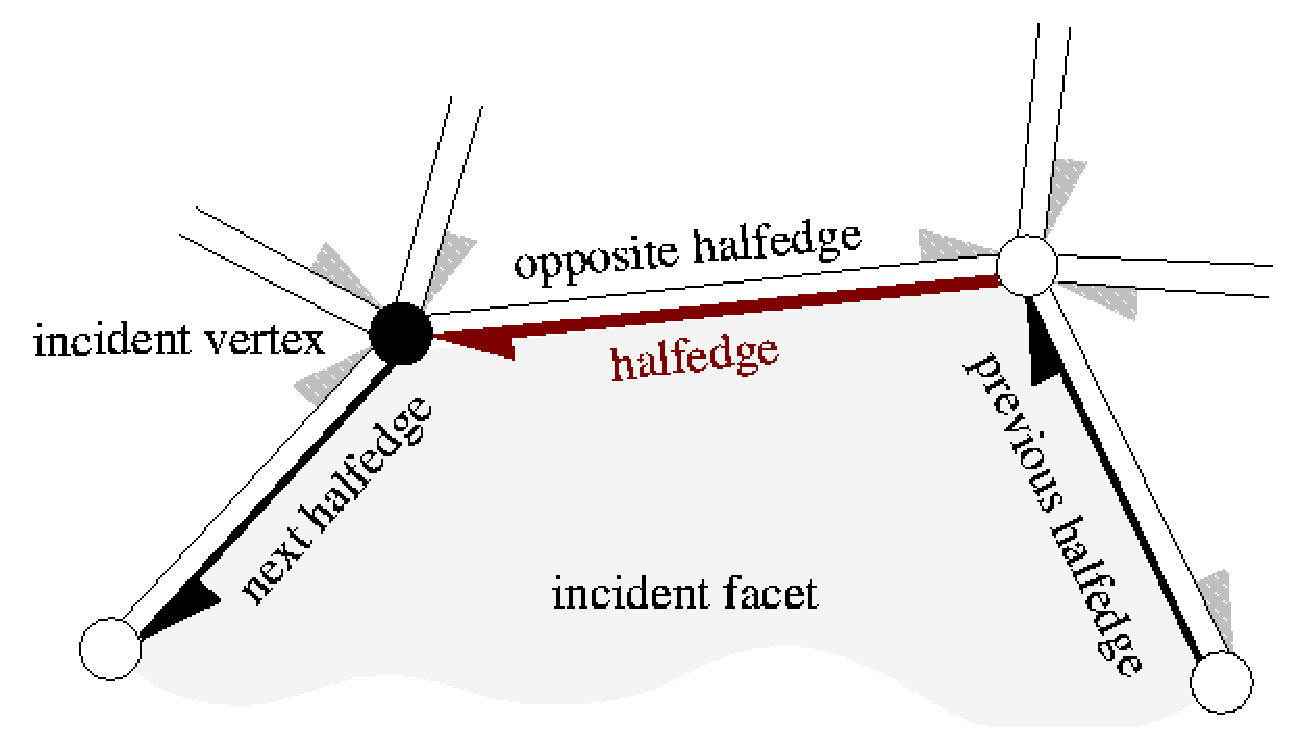
\includegraphics[width=0.4\textwidth]{Polyhedron_ref/fig/halfedge}%
%% %%       }
%% %%     \end{center}
%% %%     \vspace{-5mm}
%% %% \end{ccTexOnly}

%% %% \begin{ccHtmlOnly}
%% %%     <CENTER>
%% %%     <A HREF="fig/halfedge.gif">
%% %%         <img src="fig/halfedge_small.gif" alt="Halfedge Diagram"></A><P>
%% %%     </CENTER>
%% %% \end{ccHtmlOnly}

%% \ccInclude{CGAL/Subdivision_mask_3.h}

%% \ccParameters

%% The full template declaration of \ccClassTemplateName\ states one
%% template parameter:

%% \begin{tabbing}
%% \ccc{template <} \=\ccc{class Polyhedron_3>} \ccc{class PQQ_stencil_3;}
%% \end{tabbing}
   
%% The only parameter requires a model of 
%% the \ccc{Polyhedron_3} concept as argument. \ccc{Point_3} 
%% is required to be type-defined in \ccc{Polyhedron_3}.

%% %% \ccTypes

%% %% \ccNestedType{Traits}{traits class selected for \ccc{PolyhedronTraits_3}.}
%% %% \ccGlue
%% %% \ccNestedType{Items}{items class selected for \ccc{PolyhedronItems_3}.}
%% %% \ccGlue



%% %% % +-----------------------------------+
%% %% \begin{ccAdvanced}
%% %% \ccHeading{Types for Tagging Optional Features}

%% %% \ccNestedType{Supports_facet_plane}{\ccc{Facet::plane()}.}
%% %% \ccGlue
%% %% \ccNestedType{Supports_removal}{supports removal of individual elements.}

%% %% \end{ccAdvanced}

%% \ccCreation
%% \ccCreationVariable{P}

%% %\ccClassTemplateName\ is a functor of the three geometry stencils for
%% %subdivision surfaces based on the PQQ refinement. 
%% Default constructors are generated by the compiler.


%% % +-----------------------------------+
%% \ccHeading{Stencil Policies}
%% %\ccThree{void}{facet_node(Facet_handle f, Point& pt);}{}
%% \ccThree{void}{P.nn}{}
%% \ccThreeToTwo

%% \ccMethod{
%% void facet_node(Facet_handle f, Point& pt);
%% }{
%% define the access interface of the facet-node stencil.
%% \ccc{pt} is semantically required to be smoothed by averaging 
%% points of the neighborhood of \ccc{f}.
%% Override this function to support geometry masks for subdivisions 
%% based on the PQQ and the $\sqrt{3}$ refinement.
%% } 

%% \ccMethod{
%% void edge_node(Edge_handle e, Point& pt);
%% }{
%% define the access interface of the edge-node stencil. 
%% \ccc{pt} is semantically required to be smoothed by 
%% averaging points of the neighborhood of \ccc{e}.
%% Override this function to support geometry masks for subdivisions 
%% based on the PQQ and the PTQ refinement.
%% } 

%% \ccMethod{
%% void vertex_node(Vertex_handle v, Point& pt);
%% }{
%% define the access interface of the vertex-node stencil.
%% \ccc{pt} is semantically required to be smoothed by averaging 
%% points of the neighborhood of \ccc{v}.
%% Override this function to support geometry masks for subdivisions 
%% based on the PQQ, the PTQ and the $\sqrt{3}$ refinement.
%% } 


%% %% \begin{ccTexOnly}
%% %%     \begin{center}
%% %%       \parbox{0.636\textwidth}{%
%% %%           \includegraphics[width=0.636\textwidth]%
%% %%               {Polyhedron_ref/fig/euler_loop}%
%% %%       }
%% %%     \end{center}
%% %% \end{ccTexOnly}
%% %% \begin{ccHtmlOnly}
%% %%     <CENTER>
%% %%     <img src="fig/euler_loop.gif" alt="Euler Operator: Loop"><P>
%% %%     </CENTER>
%% %% \end{ccHtmlOnly}


%% \ccSeeAlso

%% \ccRefIdfierPage{CGAL::Subdivision_method_3<Poly>}\\
%% \ccRefIdfierPage{CGAL::DQQ_stencil_3<Poly>}\\
%% \ccRefIdfierPage{CGAL::Linear_mask_3<Poly>}\\
%% \ccRefIdfierPage{CGAL::CatmullClark_mask_3<Poly>}\\
%% \ccRefIdfierPage{CGAL::Loop_mask_3<Poly>}\\
%% \ccRefIdfierPage{CGAL::Sqrt3_mask_3<Poly>}\\

%% %\ccExample
%% %This example program instantiates a polyhedron using the default
%% %traits class and creates a tetrahedron.
%% %\ccIncludeExampleCode{Polyhedron/polyhedron_prog_simple.C}

%% \end{ccRefClass}

%% % +------------------------------------------------------------------------+
%% %%RefPage: end of main body, begin of footer
%% \ccRefPageEnd
%% % EOF



%% % +------------------------------------------------------------------------+
%% % +------------------------------------------------------------------------+
%% \ccRefPageBegin

%% %%RefPage: end of header, begin of main body
%% % +------------------------------------------------------------------------+

%% \begin{ccRefClass}{DQQ_stencil_3<Poly>}

%% \ccDefinition

%% A stencil maps an input control submesh to a node on the refined 
%% mesh. \ccClassTemplateName\ defines the policy interface of 
%% stencils of the DQQ refinement. Served as the programming guideline,
%% \ccClassTemplateName\ does not realize any specific geometry mask.

%% \ccInclude{CGAL/Subdivision_mask_3.h}

%% \ccParameters

%% The full template declaration of \ccClassTemplateName\ states one
%% template parameter:

%% \begin{tabbing}
%% \ccc{template <} \=\ccc{class Polyhedron_3>} \ccc{class DQQ_stencil_3;}
%% \end{tabbing}
   
%% The only parameter requires a model of 
%% the \ccc{Polyhedron_3} concept as argument. \ccc{Point_3} 
%% is required to be type-defined in \ccc{Polyhedron_3}.

%% \ccCreation
%% \ccCreationVariable{P}

%% Default constructors are generated by the compiler.


%% % +-----------------------------------+
%% \ccHeading{Stencil Policies}
%% %\ccThree{void}{corner_node(Halfedge_handle he, Point& pt);}{}
%% \ccThree{void}{P.nn}{}
%% \ccThreeToTwo

%% \ccMethod{
%% void corner_node(Halfedge_handle he, Point& pt);
%% }{
%% define the access interface of the corner-node stencil 
%% of the DQQ refinement. 
%% \ccc{pt} is semantically required to be smoothed by averaging 
%% points on the facet of \ccc{he}. \ccc{he} always points to the vertex 
%% that usually has the dominate mask weight.
%% }

%% \ccSeeAlso

%% \ccRefIdfierPage{CGAL::Subdivision_method_3<Poly>}\\
%% \ccRefIdfierPage{CGAL::PQQ_stencil_3<Poly>}\\
%% \ccRefIdfierPage{CGAL::DooSabin_mask_3<Poly>}\\

%% \end{ccRefClass}

%% % +------------------------------------------------------------------------+
%% %%RefPage: end of main body, begin of footer
%% \ccRefPageEnd
%% % EOF
%% % +------------------------------------------------------------------------+



%% % +------------------------------------------------------------------------+
%% % +------------------------------------------------------------------------+
%% \begin{ccRefClass}{Linear_mask_3<Poly>}

%% \ccDefinition

%% \ccClassTemplateName , inherited the policy interface from
%% \ccc{PQQ_stencil_3}, realizes the geometry masks as bi-linear 
%% averaging of nodes collected from the stencils.

%% \ccInclude{CGAL/Subdivision_mask_3.h}

%% \ccParameters

%% The full template declaration of \ccClassTemplateName\ states one
%% template parameter:

%% \begin{tabbing}
%% \ccc{template <} \=\ccc{class Polyhedron_3>} \ccc{class Linear_mask_3;}
%% \end{tabbing}
   
%% The only parameter requires a model of 
%% the \ccc{Polyhedron_3} concept as argument. 
%% \ccc{Point_3} is required to be type-defined in \ccc{Polyhedron_3}.

%% \ccCreation
%% \ccCreationVariable{P}

%% Default constructors are generated by the compiler.


%% % +-----------------------------------+
%% \ccHeading{Stencil Policies}
%% %\ccThree{void}{facet_node(Facet_handle f, Point& pt);}{}
%% \ccThree{void}{P.nn}{}
%% \ccThreeToTwo

%% \ccMethod{
%% void facet_node(Facet_handle f, Point& pt);
%% }{
%% assign the centroid of \ccc{f} to \ccc{pt}.
%% }

%% \ccMethod{
%% void edge_node(Edge_handle e, Point& pt);
%% }{
%% assign the mid-point of \ccc{e} to \ccc{pt}.
%% }

%% \ccMethod{
%% void vertex_node(Vertex_handle v, Point& pt);
%% }{
%% assign the point on \ccc{v} to \ccc{pt}.
%% }

%% \ccSeeAlso

%% \ccRefIdfierPage{CGAL::Subdivision_method_3<Poly>}\\
%% \ccRefIdfierPage{CGAL::PQQ_stencil_3<Poly>}\\
%% \ccRefIdfierPage{CGAL::CatmullClark_mask_3<Poly>}\\
%% \ccRefIdfierPage{CGAL::Loop_mask_3<Poly>}\\
%% \ccRefIdfierPage{CGAL::Sqrt3_mask_3<Poly>}\\

%% \end{ccRefClass}

%% % +------------------------------------------------------------------------+
%% %%RefPage: end of main body, begin of footer
%% \ccRefPageEnd
%% % EOF
%% % +------------------------------------------------------------------------+



% +------------------------------------------------------------------------+
% +------------------------------------------------------------------------+
\begin{ccRefClass}{CatmullClark_mask_3<Polyhedron_3>}

\ccDefinition

A stencil determines a source neighborhood 
whose points contribute to the position of a refined point.
The geometry mask of a stencil specifies
the computation on the nodes of the stencil.
\ccClassTemplateName\ implements the geometry masks of 
Catmull-Clark subdivision on a \ccc{Polyhedron_3<Cartesian>}.

\ccInclude{CGAL/Subdivision_mask_3.h}

\ccParameters

The full template declaration of \ccClassTemplateName\ states one
template parameter:

\begin{tabbing}
\ccc{template <} \=\ccc{class Polyhedron_3>} \ccc{class CatmullClark_mask_3;}
\end{tabbing}
   
The only parameter requires a \ccc{Polyhedron_3} as the argument. The
\ccc{Polyhedron_3} should be specialized with the \ccc{Cartesian}
kernel, which defines the \ccc{Point_3} for the vertices.

\ccCreation
\ccCreationVariable{CC}

\ccConstructor{CatmullClark_mask_3<Polyhedron_3>();}{default constructor.}

% +-----------------------------------+
\ccHeading{Stencil functions}
%\ccThree{void}{facet_node(Facet_handle f, Point& pt);}{}
\ccThree{void}{CC.nn}{}
\ccThreeToTwo

\ccMethod{
void facet_node(Facet_handle f, Point_3& pt);
}{
computes the Catmull-Clark facet-point \ccc{pt} of the facet \ccc{f}.
}

\ccMethod{
void edge_node(Edge_handle e, Point_3& pt);
}{
computes the Catmull-Clark edge-point \ccc{pt} of the edge \ccc{e}.
}

\ccMethod{
void vertex_node(Vertex_handle v, Point_3& pt);
}{
computes the Catmull-Clark vertex-point \ccc{pt} of the vertex \ccc{v}.
}

\ccMethod{
void border_node(Halfedge_handle e, Point_3& ept, Point_3& vpt);
}{
computes the Catmull-Clark edge-point \ccc{ept} and the 
Catmull-Clark vertex-point \ccc{vpt} of the border edge \ccc{e}.
}

\begin{ccTexOnly}
  \begin{center}
    \parbox{0.6\textwidth}{%
      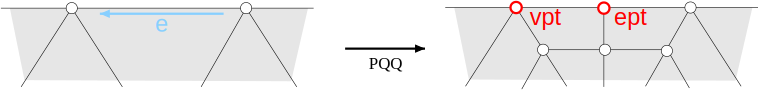
\includegraphics[width=0.6\textwidth]{Subdivision_method_3_ref/FIG/CCBorderMask}%
    }\\ \vspace{0.5cm}
  \end{center}
\end{ccTexOnly}

\begin{ccHtmlOnly}
    <CENTER>
      <img src="FIG/CCBorderMask.png" alt="PQQ stencil of border nodes"></A><P>
    </CENTER>
\end{ccHtmlOnly}

\ccSeeAlso

\ccRefIdfierPage{CGAL::Subdivision_method_3}\\
%%\ccRefIdfierPage{CGAL::PQQ_stencil_3<Polyhedron_3>}\\
%%\ccRefIdfierPage{CGAL::Linear_mask_3<Polyhedron_3>}\\

\end{ccRefClass}

% +------------------------------------------------------------------------+
%%RefPage: end of main body, begin of footer
\ccRefPageEnd
% EOF
% +------------------------------------------------------------------------+


% +------------------------------------------------------------------------+
% +------------------------------------------------------------------------+
\begin{ccRefClass}{Loop_mask_3<Polyhedron_3>}

\ccDefinition

A stencil determines a source neighborhood 
whose points contribute to the position of a refined point.
The geometry mask of a stencil specifies
the computation on the nodes of the stencil.
\ccClassTemplateName\ implements the geometry masks of 
Loop subdivision on a triangulated \ccc{Polyhedron_3<Cartesian>}.

\ccInclude{CGAL/Subdivision_mask_3.h}

\ccParameters

The full template declaration of \ccClassTemplateName\ states one
template parameter:

\begin{tabbing}
\ccc{template <} \=\ccc{class Polyhedron_3>} \ccc{class Loop_mask_3;}
\end{tabbing}
   
The only parameter requires a \ccc{Polyhedron_3} as the argument. The
\ccc{Polyhedron_3} should be specialized with the \ccc{Cartesian}
kernel, which defines the \ccc{Point_3} for the vertices.

\ccCreation
\ccCreationVariable{L}

\ccConstructor{Loop_mask_3<Polyhedron_3>();}{default constructor.}

% +-----------------------------------+
\ccHeading{Stencil functions}
%\ccThree{void}{edge_node(Edge_handle e, Point& pt);}{}
\ccThree{void}{L.nn}{}
\ccThreeToTwo

\ccMethod{
void edge_node(Edge_handle e, Point_3& pt);
}{
computes the Loop edge-point \ccc{pt} of the edge \ccc{e}.
}

\ccMethod{
void vertex_node(Vertex_handle v, Point_3& pt);
}{
computes the Loop vertex-point \ccc{pt} of the vertex \ccc{v}.
}

\ccMethod{
void border_node(Halfedge_handle e, Point_3& ept, Point_3& vpt);
}{
computes the Loop edge-point \ccc{ept} and the 
Loop vertex-point \ccc{vpt} of the border edge \ccc{e}.
}

\begin{ccTexOnly}
  \begin{center}
    \parbox{0.6\textwidth}{%
      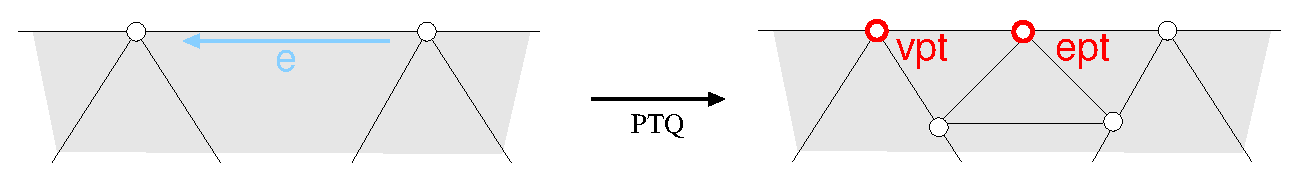
\includegraphics[width=0.6\textwidth]{Subdivision_method_3_ref/FIG/LoopBorderMask}%
    }\\ \vspace{0.5cm}
  \end{center}
\end{ccTexOnly}

\begin{ccHtmlOnly}
    <CENTER>
      <img src="FIG/LoopBorderMask.png" alt="PTQ stencil of border nodes"></A><P>
    </CENTER>
\end{ccHtmlOnly}

\ccSeeAlso

\ccRefIdfierPage{CGAL::Subdivision_method_3}\\
%%\ccRefIdfierPage{CGAL::PQQ_stencil_3<Poly>}\\

\end{ccRefClass}

% +------------------------------------------------------------------------+
%%RefPage: end of main body, begin of footer
\ccRefPageEnd
% EOF
% +------------------------------------------------------------------------+


% +------------------------------------------------------------------------+
% +------------------------------------------------------------------------+
\begin{ccRefClass}{DooSabin_mask_3<Polyhedron_3>}

\ccDefinition

A stencil determines a source neighborhood 
whose points contribute to the position of a refined point.
The geometry mask of a stencil specifies
the computation on the nodes of the stencil.
\ccClassTemplateName\ implements the geometry masks of 
Doo-Sabin subdivision on a \ccc{Polyhedron_3<Cartesian>}.

\ccInclude{CGAL/Subdivision_mask_3.h}

\ccParameters

The full template declaration of \ccClassTemplateName\ states one
template parameter:

\begin{tabbing}
\ccc{template <} \=\ccc{class Polyhedron_3>} \ccc{class DooSabin_mask_3;}
\end{tabbing}
   
The only parameter requires a \ccc{Polyhedron_3} as the argument. The
\ccc{Polyhedron_3} should be specialized with the \ccc{Cartesian}
kernel, which defines the \ccc{Point_3} for the vertices.

\ccCreation
\ccCreationVariable{DS}

\ccConstructor{DooSabin_mask_3<Polyhedron_3>();}{default constructor.}

% +-----------------------------------+
\ccHeading{Stencil functions}
%\ccThree{void}{corner_node(Halfedge_handle he, Point& pt);}{}
\ccThree{void}{DS.nn}{}
\ccThreeToTwo

\ccMethod{
void corner_node(Halfedge_handle he, Point_3& pt);
}{
computes the Doo-Sabin point \ccc{pt} of the vertex pointed
by the halfedge \ccc{he}.
}

\begin{ccTexOnly}
  \begin{center}
    \parbox{0.6\textwidth}{%
      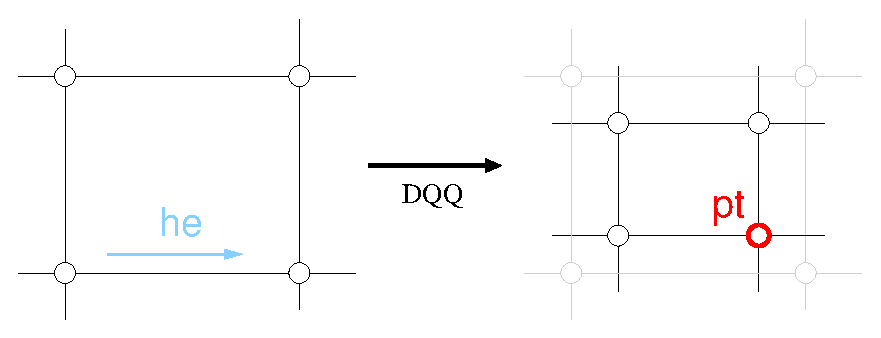
\includegraphics[width=0.45\textwidth]{Subdivision_method_3_ref/FIG/DSCornerMask}%
    }\\ \vspace{0.5cm}
  \end{center}
\end{ccTexOnly}

\begin{ccHtmlOnly}
    <CENTER>
      <img src="FIG/DSCornerMask.png" alt="DQQ corner stencil"></A><P>
    </CENTER>
\end{ccHtmlOnly}

\ccSeeAlso

\ccRefIdfierPage{CGAL::Subdivision_method_3}\\
%%\ccRefIdfierPage{CGAL::DQQ_stencil_3<Poly>}\\

\end{ccRefClass}

% +------------------------------------------------------------------------+
%%RefPage: end of main body, begin of footer
\ccRefPageEnd
% EOF
% +------------------------------------------------------------------------+


% +------------------------------------------------------------------------+
% +------------------------------------------------------------------------+
\begin{ccRefClass}{Sqrt3_mask_3<Polyhedron_3>}

\ccDefinition

A stencil determines a source neighborhood 
whose points contribute to the position of a refined point.
The geometry mask of a stencil specifies
the computation on the nodes of the stencil.
\ccClassTemplateName\ implements the geometry masks of 
$\sqrt{3}$ subdivision on a triangulated 
\ccc{Polyhedron_3<Cartesian>}.

\ccInclude{CGAL/Subdivision_mask_3.h}

\ccParameters

The full template declaration of \ccClassTemplateName\ states one
template parameter:

\begin{tabbing}
\ccc{template <} \=\ccc{class Polyhedron_3>} \ccc{class Sqrt3_mask_3;}
\end{tabbing}
   
The only parameter requires a \ccc{Polyhedron_3} as the argument. The
\ccc{Polyhedron_3} should be specialized with the \ccc{Cartesian}
kernel, which defines the \ccc{Point_3} for the vertices.

\ccCreation
\ccCreationVariable{S}

\ccConstructor{Sqrt3_mask_3<Polyhedron_3>();}{default constructor.}

% +-----------------------------------+
\ccHeading{Stencil functions}
%\ccThree{void}{facet_node(Facet_handle f, Point& pt);}{}
\ccThree{void}{S.nn}{}
\ccThreeToTwo

\ccMethod{
void facet_node(Facet_handle f, Point_3& pt);
}{
computes the $\sqrt{3}$ facet-point \ccc{pt} of the facet \ccc{f}.
}

\ccMethod{
void vertex_node(Vertex_handle v, Point& pt);
}{
computes the $\sqrt{3}$ vertex-point \ccc{pt} of the vertex \ccc{v}.
}

\ccSeeAlso

\ccRefIdfierPage{CGAL::Subdivision_method_3}\\
%\ccRefIdfierPage{CGAL::PQQ_stencil_3<Poly>}\\
%\ccRefIdfierPage{CGAL::Linear_mask_3<Poly>}\\

\end{ccRefClass}

% +------------------------------------------------------------------------+
%%RefPage: end of main body, begin of footer
\ccRefPageEnd
% EOF
% +------------------------------------------------------------------------+

